\documentclass[10pt]{article}
\usepackage[polish]{babel}
\usepackage[utf8]{inputenc}
\usepackage[T1]{fontenc}
\usepackage{graphicx}
\usepackage[export]{adjustbox}
\graphicspath{ {./images/} }
\usepackage{amsmath}
\usepackage{amsfonts}
\usepackage{amssymb}
\usepackage[version=4]{mhchem}
\usepackage{stmaryrd}
\usepackage{multirow}

\title{EGZAMIN MATURALNY \\
 Z MATEMATYKI }

\author{}
\date{}


\begin{document}
\maketitle
Arkusz zawiera informacje prawnie chronione do momentu rozpoczęcia egzaminu.\\
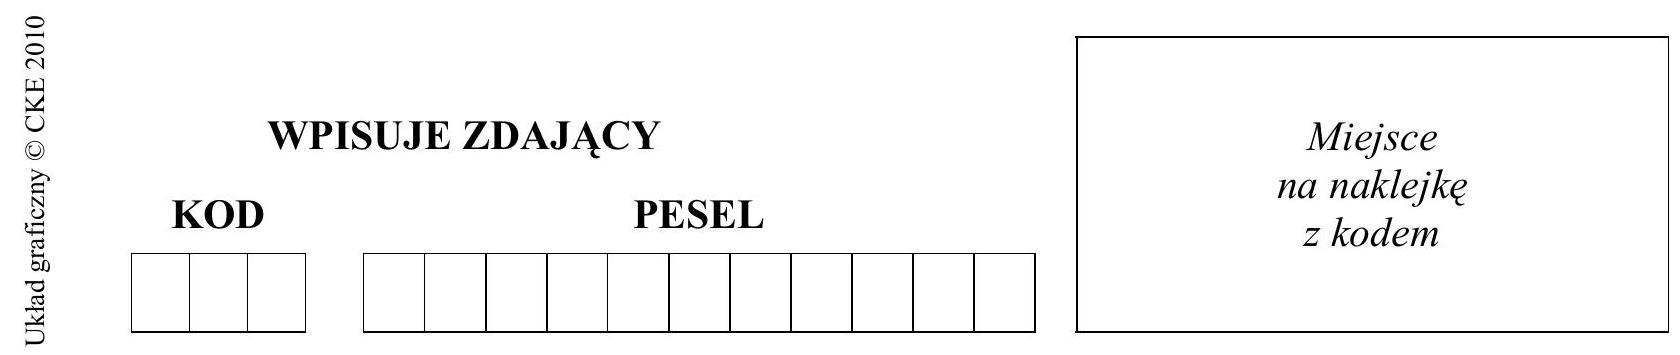
\includegraphics[max width=\textwidth, center]{2024_11_21_caf6b2e64dd65c9b24eeg-01}

\section*{POZIOM PODSTAWOWY}
MAJ 2010

\begin{enumerate}
  \item Sprawdź, czy arkusz egzaminacyjny zawiera 20 stron (zadania 1-34). Ewentualny brak zgłoś przewodniczącemu zespołu nadzorującego egzamin.
  \item Rozwiązania zadań i odpowiedzi wpisuj w miejscu na to przeznaczonym.
  \item Odpowiedzi do zadań zamkniętych (1-25) przenieś na kartę odpowiedzi, zaznaczając je w części karty przeznaczonej dla zdającego. Zamaluj \(\square\) pola do tego przeznaczone. Błędne zaznaczenie otocz kółkiem i zaznacz właściwe.
  \item Pamiętaj, że pominięcie argumentacji lub istotnych obliczeń w rozwiązaniu zadania otwartego (26-34) może
\end{enumerate}

Czas pracy: 170 minut\\
spowodować, że za to rozwiązanie nie będziesz mógł dostać pełnej liczby punktów.\\
5. Pisz czytelnie i używaj tylko długopisu lub pióra z czarnym tuszem lub atramentem.\\
6. Nie używaj korektora, a błędne zapisy wyraźnie przekreśl.\\
7. Pamiętaj, że zapisy w brudnopisie nie będą oceniane.\\
8. Możesz korzystać z zestawu wzorów matematycznych, cyrkla i linijki oraz kalkulatora.\\
9. Na karcie odpowiedzi wpisz swój numer PESEL i przyklej naklejkę z kodem.\\
10. Nie wpisuj żadnych znaków w części przeznaczonej dla egzaminatora.

Liczba punktów do uzyskania: 50

MMA-P1\\
1P-102

\section*{ZADANIA ZAMKNIĘTE}
W zadaniach od 1. do 25. wybierz izaznacz na karcie odpowiedzi poprawną odpowiedź.

\section*{Zadanie 1. (1 pkt)}
Wskaż rysunek, na którym jest przedstawiony zbiór rozwiązań nierówności \(|x+7|>5\).\\
A.\\
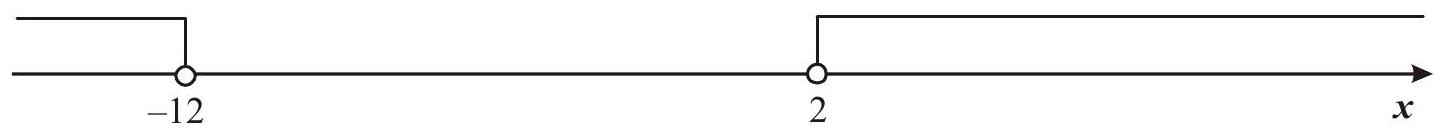
\includegraphics[max width=\textwidth, center]{2024_11_21_caf6b2e64dd65c9b24eeg-02}\\
B.\\
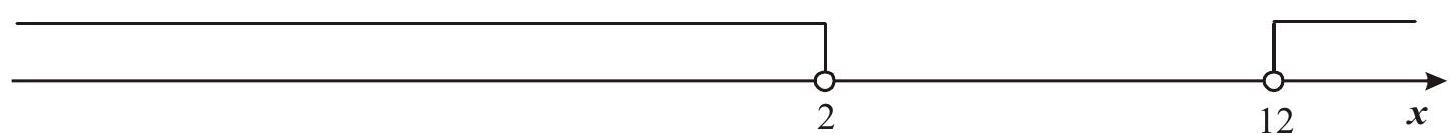
\includegraphics[max width=\textwidth, center]{2024_11_21_caf6b2e64dd65c9b24eeg-02(2)}\\
C.\\
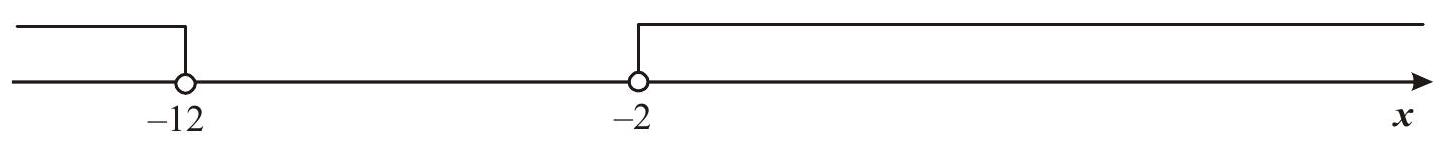
\includegraphics[max width=\textwidth, center]{2024_11_21_caf6b2e64dd65c9b24eeg-02(3)}\\
D.\\
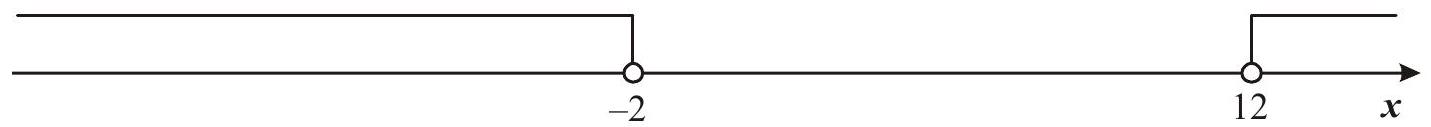
\includegraphics[max width=\textwidth, center]{2024_11_21_caf6b2e64dd65c9b24eeg-02(1)}

Zadanie 2. (1 pkt)\\
Spodnie po obniżce ceny o \(30 \%\) kosztują 126 zł. Ile kosztowały spodnie przed obniżką?\\
A. \(163,80 \mathrm{zt}\)\\
B. 180 zt\\
C. 294 zl\\
D. 420 zl

\section*{Zadanie 3. (1 pkt)}
Liczba \(\left(\frac{2^{-2} \cdot 3^{-1}}{2^{-1} \cdot 3^{-2}}\right)^{0}\) jest równa\\
A. 1\\
B. 4\\
C. 9\\
D. 36

Zadanie 4. (1 pkt)\\
Liczba \(\log _{4} 8+\log _{4} 2\) jest równa\\
A. 1\\
B. 2\\
C. \(\log _{4} 6\)\\
D. \(\log _{4} 10\)

\section*{Zadanie 5. (1 pkt)}
Dane są wielomiany \(W(x)=-2 x^{3}+5 x^{2}-3\) oraz \(P(x)=2 x^{3}+12 x\). Wielomian \(W(x)+P(x)\) jest równy\\
A. \(5 x^{2}+12 x-3\)\\
B. \(4 x^{3}+5 x^{2}+12 x-3\)\\
C. \(4 x^{6}+5 x^{2}+12 x-3\)\\
D. \(4 x^{3}+12 x^{2}-3\)

\section*{BRUDNOPIS}
\begin{center}

\includegraphics[max width=\textwidth]{2024_11_21_caf6b2e64dd65c9b24eeg-03}
\end{center}

\section*{Zadanie 6. (1 pkt)}
Rozwiązaniem równania \(\frac{3 x-1}{7 x+1}=\frac{2}{5}\) jest\\
A. 1\\
B. \(\frac{7}{3}\)\\
C. \(\frac{4}{7}\)\\
D. 7

\section*{Zadanie 7. (1 pkt)}
Do zbioru rozwiązań nierówności \((x-2)(x+3)<0\) należy liczba\\
A. 9\\
B. 7\\
C. 4\\
D. 1

\section*{Zadanie 8. (1 pkt)}
Wykresem funkcji kwadratowej \(f(x)=-3 x^{2}+3\) jest parabola o wierzchołku w punkcie\\
A. \((3,0)\)\\
B. \((0,3)\)\\
C. \((-3,0)\)\\
D. \((0,-3)\)

\section*{Zadanie 9. (1 pkt)}
Prosta o równaniu \(y=-2 x+(3 m+3)\) przecina w układzie współrzędnych oś \(O y\) w punkcie \((0,2)\). Wtedy\\
A. \(m=-\frac{2}{3}\)\\
B. \(m=-\frac{1}{3}\)\\
C. \(m=\frac{1}{3}\)\\
D. \(m=\frac{5}{3}\)

\section*{Zadanie 10. (1 pkt)}
Na rysunku jest przedstawiony wykres funkcji \(y=f(x)\).\\
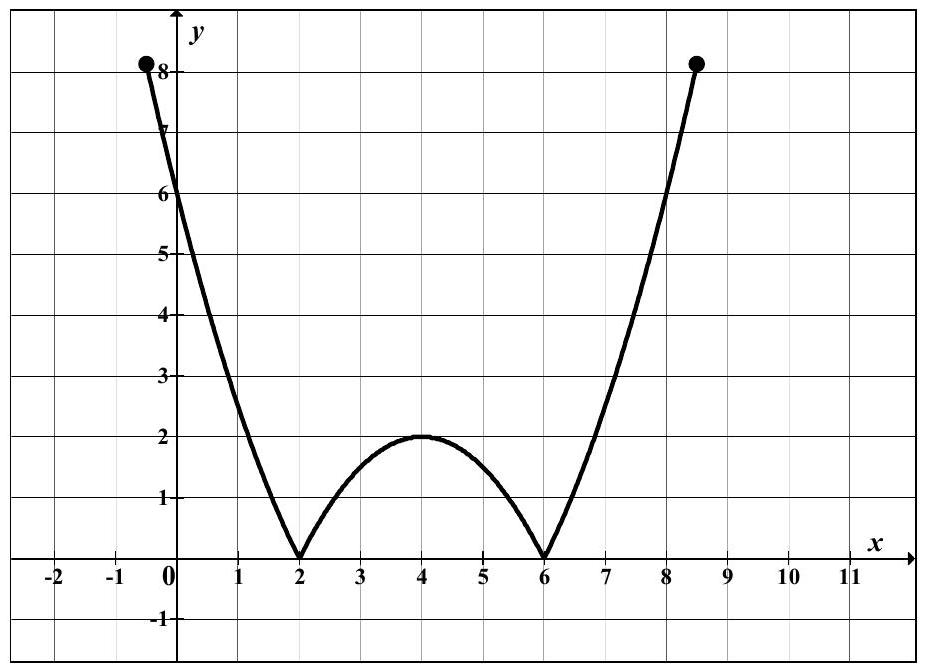
\includegraphics[max width=\textwidth, center]{2024_11_21_caf6b2e64dd65c9b24eeg-04}

Które równanie ma dokładnie trzy rozwiązania?\\
A. \(f(x)=0\)\\
B. \(f(x)=1\)\\
C. \(f(x)=2\)\\
D. \(f(x)=3\)

\section*{Zadanie 11. (1 pkt)}
W ciagu arytmetycznym \(\left(a_{n}\right)\) dane sa: \(a_{3}=13\) i \(a_{5}=39\). Wtedy wyraz \(a_{1}\) jest równy\\
A. 13\\
B. 0\\
C. -13\\
D. -26

\section*{Zadanie 12. (1 pkt)}
W ciagu geometrycznym \(\left(a_{n}\right)\) dane sa: \(a_{1}=3\) i \(a_{4}=24\). Iloraz tego ciagu jest równy\\
A. 8\\
B. 2\\
C. \(\frac{1}{8}\)\\
D. \(-\frac{1}{2}\)

\section*{BRUDNOPIS}
\begin{center}

\includegraphics[max width=\textwidth]{2024_11_21_caf6b2e64dd65c9b24eeg-05}
\end{center}

\section*{Zadanie 13. (1 pkt)}
Liczba przekątnych siedmiokąta foremnego jest równa\\
A. 7\\
B. 14\\
C. 21\\
D. 28

\section*{Zadanie 14. (1 pkt)}
Kąt \(\alpha\) jest ostry i \(\sin \alpha=\frac{3}{4}\). Wartość wyrażenia \(2-\cos ^{2} \alpha\) jest równa\\
A. \(\frac{25}{16}\)\\
B. \(\frac{3}{2}\)\\
C. \(\frac{17}{16}\)\\
D. \(\frac{31}{16}\)

Zadanie 15. (1 pkt)\\
Okragg opisany na kwadracie ma promień 4. Długość boku tego kwadratu jest równa\\
A. \(4 \sqrt{2}\)\\
B. \(2 \sqrt{2}\)\\
C. 8\\
D. 4

\section*{Zadanie 16. (1 pkt)}
Podstawa trójkąta równoramiennego ma długość 6, a ramię ma długość 5. Wysokość opuszczona na podstawę ma długość\\
A. 3\\
B. 4\\
C. \(\sqrt{34}\)\\
D. \(\sqrt{61}\)

\section*{Zadanie 17. (1 pkt)}
Odcinki \(A B\) i \(D E\) są równoległe. Długości odcinków \(C D, D E\) i \(A B\) są odpowiednio równe 1, 3 i 9. Długość odcinka \(A D\) jest równa\\
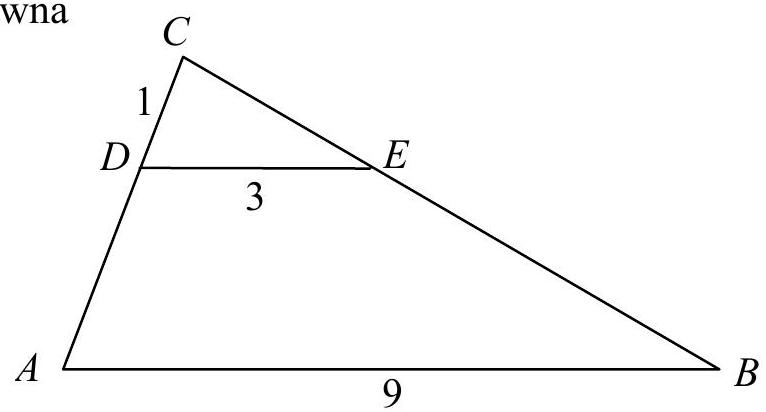
\includegraphics[max width=\textwidth, center]{2024_11_21_caf6b2e64dd65c9b24eeg-06(1)}\\
A. 2\\
B. 3\\
C. 5\\
D. 6

Zadanie 18. (1 pkt)\\
Punkty \(A, B, C\) leżące na okręgu o środku \(S\) są wierzchołkami trójkąta równobocznego. Miara zaznaczonego na rysunku kąta środkowego \(A S B\) jest równa\\
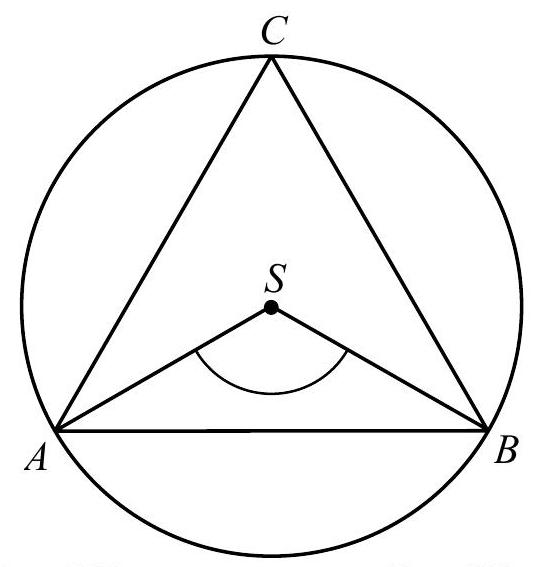
\includegraphics[max width=\textwidth, center]{2024_11_21_caf6b2e64dd65c9b24eeg-06}\\
A. \(120^{\circ}\)\\
B. \(90^{\circ}\)\\
C. \(60^{\circ}\)\\
D. \(30^{\circ}\)

\section*{BRUDNOPIS}
\begin{center}

\includegraphics[max width=\textwidth]{2024_11_21_caf6b2e64dd65c9b24eeg-07}
\end{center}

\section*{Zadanie 19. (1 pkt)}
\begin{center}
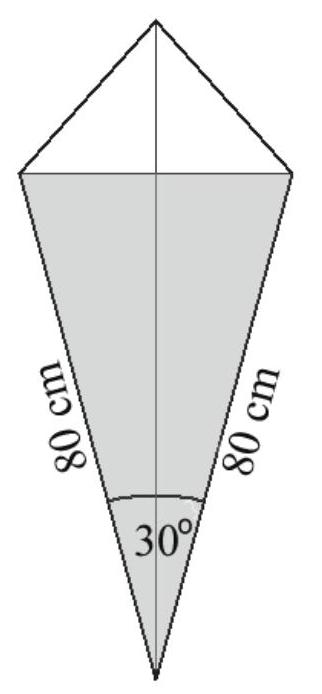
\includegraphics[max width=\textwidth]{2024_11_21_caf6b2e64dd65c9b24eeg-08}
\end{center}

Latawiec ma wymiary podane na rysunku. Powierzchnia zacieniowanego trójkąta jest równa\\
A. \(3200 \mathrm{~cm}^{2}\)\\
B. \(6400 \mathrm{~cm}^{2}\)\\
C. \(1600 \mathrm{~cm}^{2}\)\\
D. \(800 \mathrm{~cm}^{2}\)

\section*{Zadanie 20. (1 pkt)}
Współczynnik kierunkowy prostej równoległej do prostej o równaniu \(y=-3 x+5\) jest równy:\\
A. \(-\frac{1}{3}\)\\
B. -3\\
C. \(\frac{1}{3}\)\\
D. 3

\section*{Zadanie 21. (1 pkt)}
Wskaż równanie okręgu o promieniu 6.\\
A. \(x^{2}+y^{2}=3\)\\
B. \(x^{2}+y^{2}=6\)\\
C. \(x^{2}+y^{2}=12\)\\
D. \(x^{2}+y^{2}=36\)

\section*{Zadanie 22. (1 pkt)}
Punkty \(A=(-5,2)\) i \(B=(3,-2)\) są wierzchołkami trójkąta równobocznego \(A B C\). Obwód tego trójkąta jest równy\\
A. 30\\
B. \(4 \sqrt{5}\)\\
C. \(12 \sqrt{5}\)\\
D. 36

\section*{Zadanie 23. (1 pkt)}
Pole powierzchni całkowitej prostopadłościanu o wymiarach \(5 \times 3 \times 4\) jest równe\\
A. 94\\
B. 60\\
C. 47\\
D. 20

\section*{Zadanie 24. (1 pkt)}
Ostrosłup ma 18 wierzchołków. Liczba wszystkich krawędzi tego ostrosłupa jest równa\\
A. 11\\
B. 18\\
C. 27\\
D. 34

\section*{Zadanie 25. (1 pkt)}
Średnia arytmetyczna dziesięciu liczb \(x, 3,1,4,1,5,1,4,1,5\) jest równa 3 . Wtedy\\
A. \(x=2\)\\
B. \(x=3\)\\
C. \(x=4\)\\
D. \(x=5\)

\section*{BRUDNOPIS}
\begin{center}

\includegraphics[max width=\textwidth]{2024_11_21_caf6b2e64dd65c9b24eeg-09}
\end{center}

\section*{ZADANIA OTWARTE}
\section*{Rozwiqzania zadań o numerach od 26. do 34. nalė̇̀y zapisać \(\boldsymbol{w}\) wyznaczonych miejscach pod treścia zadania.}
\section*{Zadanie 26. (2 pkt)}
Rozwiąż nierówność \(x^{2}-x-2 \leq 0\).\\

\includegraphics[max width=\textwidth, center]{2024_11_21_caf6b2e64dd65c9b24eeg-10(1)}

Odpowiedź:

\section*{Zadanie 27. (2 pkt)}
Rozwiąż równanie \(x^{3}-7 x^{2}-4 x+28=0\).\\

\includegraphics[max width=\textwidth, center]{2024_11_21_caf6b2e64dd65c9b24eeg-10}

Odpowiedź:

\section*{Zadanie 28. (2 pkt)}
Trójkąty prostokątne równoramienne \(A B C\) i \(C D E\) są położone tak, jak na poniższym rysunku (w obu trójkątach kąt przy wierzchołku \(C\) jest prosty). Wykaż, że \(|A D|=|B E|\).\\
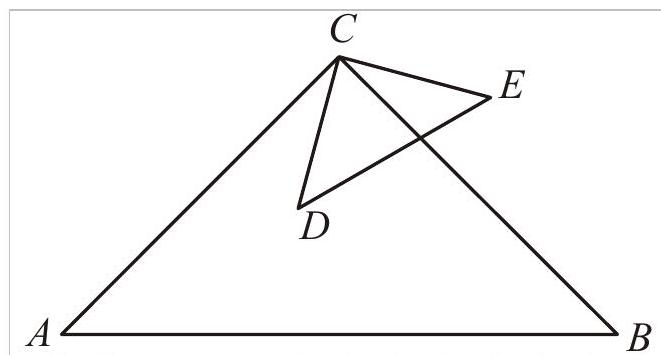
\includegraphics[max width=\textwidth, center]{2024_11_21_caf6b2e64dd65c9b24eeg-11}

\begin{center}
\begin{tabular}{|c|l|c|c|c|}
\hline
\multirow{3}{*}{\begin{tabular}{c}
Wypelnia \\
egzaminator \\
\end{tabular}} & Nr zadania & 26. & 27. & 28. \\
\cline { 2 - 5 }
 & Maks. liczba pkt & \(\mathbf{2}\) & \(\mathbf{2}\) & \(\mathbf{2}\) \\
\cline { 2 - 5 }
 & Uzyskana liczba pkt &  &  &  \\
\hline
\end{tabular}
\end{center}

Zadanie 29. (2 pkt)\\
Kąt \(\alpha\) jest ostry i \(\operatorname{tg} \alpha=\frac{5}{12}\). Oblicz \(\cos \alpha\).

\begin{center}
\begin{tabular}{|c|c|c|c|c|c|c|c|c|c|c|c|c|c|c|c|c|c|c|c|c|c|c|c|c|c|c|c|c|c|c|c|}
\hline
 &  &  &  &  &  &  &  &  &  &  &  &  &  &  &  &  &  &  &  &  &  &  &  &  &  &  &  &  &  &  &  \\
\hline
 &  &  &  &  &  &  &  &  &  &  &  &  &  &  &  &  &  &  &  &  &  &  &  &  &  &  &  &  &  &  &  \\
\hline
 &  &  &  &  &  &  &  &  &  &  &  &  &  &  &  &  &  &  &  &  &  &  &  &  &  &  &  &  &  &  &  \\
\hline
 &  &  &  &  &  &  &  &  &  &  &  &  &  &  &  &  &  &  &  &  &  &  &  &  &  &  &  &  &  &  &  \\
\hline
 &  &  &  &  &  &  &  &  &  &  &  &  &  &  &  &  &  &  &  &  &  &  &  &  &  &  &  &  &  &  &  \\
\hline
 &  &  &  &  &  &  &  &  &  &  &  &  &  &  &  &  &  &  &  &  &  &  &  &  &  &  &  &  &  &  &  \\
\hline
 &  &  &  &  &  &  &  &  &  &  &  &  &  &  &  &  &  &  &  &  &  &  &  &  &  &  &  &  &  &  &  \\
\hline
 &  &  &  &  &  &  &  &  &  &  &  &  &  &  &  &  &  &  &  &  &  &  &  &  &  &  &  &  &  &  &  \\
\hline
 &  &  &  &  &  &  &  &  &  &  &  &  &  &  &  &  &  &  &  &  &  &  &  &  &  &  &  &  &  &  &  \\
\hline
 &  &  &  &  &  &  &  &  &  &  &  &  &  &  &  &  &  &  &  &  &  &  &  &  &  &  &  &  &  &  &  \\
\hline
 &  &  &  &  &  &  &  &  &  &  &  &  &  &  &  &  &  &  &  &  &  &  &  &  &  &  &  &  &  &  &  \\
\hline
 &  &  &  &  &  &  &  &  &  &  &  &  &  &  &  &  &  &  &  &  &  &  &  &  &  &  &  &  &  &  &  \\
\hline
 &  &  &  &  &  &  &  &  &  &  &  &  &  &  &  &  &  &  &  &  &  &  &  &  &  &  &  &  &  &  &  \\
\hline
 &  &  &  &  &  &  &  &  &  &  &  &  &  &  &  &  &  &  &  &  &  &  &  &  &  &  &  &  &  &  &  \\
\hline
 &  &  &  &  &  &  &  &  &  &  &  &  &  &  &  &  &  &  &  &  &  &  &  &  &  &  &  &  &  &  &  \\
\hline
 &  &  &  &  &  &  &  &  &  &  &  &  &  &  &  &  &  &  &  &  &  &  &  &  &  &  &  &  &  &  &  \\
\hline
 &  &  &  &  &  &  &  &  &  &  &  &  &  &  &  &  &  &  &  &  &  &  &  &  &  &  &  &  &  &  &  \\
\hline
 &  &  &  &  &  &  &  &  &  &  &  &  &  &  &  &  &  &  &  &  &  &  &  &  &  &  &  &  &  &  &  \\
\hline
 &  &  &  &  &  &  &  &  &  &  &  &  &  &  &  &  &  &  &  &  &  &  &  &  &  &  &  &  &  &  &  \\
\hline
\end{tabular}
\end{center}

\section*{Odpowiedź:}
\section*{Zadanie 30. (2 pkt)}
Wykaż, że jeśli \(a>0\), to \(\frac{a^{2}+1}{a+1} \geq \frac{a+1}{2}\).

\begin{center}
\begin{tabular}{|c|c|c|c|c|c|c|c|c|c|c|c|c|c|c|c|c|c|c|c|c|c|c|c|c|c|c|c|c|c|c|}
\hline
 &  &  &  &  &  &  &  &  &  &  &  &  &  &  &  &  &  &  &  &  &  &  &  &  &  &  &  &  &  &  \\
\hline
 &  &  &  &  &  &  &  &  &  &  &  &  &  &  &  &  &  &  &  &  &  &  &  &  &  &  &  &  &  &  \\
\hline
 &  &  &  &  &  &  &  &  &  &  &  &  &  &  &  &  &  &  &  &  &  &  &  &  &  &  &  &  &  &  \\
\hline
 &  &  &  &  &  &  &  &  &  &  &  &  &  &  &  &  &  &  &  &  &  &  &  &  &  &  &  &  &  &  \\
\hline
 &  &  &  &  &  &  &  &  &  &  &  &  &  &  &  &  &  &  &  &  &  &  &  &  &  &  &  &  &  &  \\
\hline
 &  &  &  &  &  &  &  &  &  &  &  &  &  &  &  &  &  &  &  &  &  &  &  &  &  &  &  &  &  &  \\
\hline
 &  &  &  &  &  &  &  &  &  &  &  &  &  &  &  &  &  &  &  &  &  &  &  &  &  &  &  &  &  &  \\
\hline
 &  &  &  &  &  &  &  &  &  &  &  &  &  &  &  &  &  &  &  &  &  &  &  &  &  &  &  &  &  &  \\
\hline
 &  &  &  &  &  &  &  &  &  &  &  &  &  &  &  &  &  &  &  &  &  &  &  &  &  &  &  &  &  &  \\
\hline
 &  &  &  &  &  &  &  &  &  &  &  &  &  &  &  &  &  &  &  &  &  &  &  &  &  &  &  &  &  &  \\
\hline
 &  &  &  &  &  &  &  &  &  &  &  &  &  &  &  &  &  &  &  &  &  &  &  &  &  &  &  &  &  &  \\
\hline
 &  &  &  &  &  &  &  &  &  &  &  &  &  &  &  &  &  &  &  &  &  &  &  &  &  &  &  &  &  &  \\
\hline
 &  &  &  &  &  &  &  &  &  &  &  &  &  &  &  &  &  &  &  &  &  &  &  &  &  &  &  &  &  &  \\
\hline
 &  &  &  &  &  &  &  &  &  &  &  &  &  &  &  &  &  &  &  &  &  &  &  &  &  &  &  &  &  &  \\
\hline
 &  &  &  &  &  &  &  &  &  &  &  &  &  &  &  &  &  &  &  &  &  &  &  &  &  &  &  &  &  &  \\
\hline
 &  &  &  &  &  &  &  &  &  &  &  &  &  &  &  &  &  &  &  &  &  &  &  &  &  &  &  &  &  &  \\
\hline
 &  &  &  &  &  &  &  &  &  &  &  &  &  &  &  &  &  &  &  &  &  &  &  &  &  &  &  &  &  &  \\
\hline
 &  &  &  &  &  &  &  &  &  &  &  &  &  &  &  &  &  &  &  &  &  &  &  &  &  &  &  &  &  &  \\
\hline
 &  &  &  &  &  &  &  &  &  &  &  &  &  &  &  &  &  &  &  &  &  &  &  &  &  &  &  &  &  &  \\
\hline
 &  &  &  &  &  &  &  &  &  &  &  &  &  &  &  &  &  &  &  &  &  &  &  &  &  &  &  &  &  &  \\
\hline
\end{tabular}
\end{center}

\section*{Zadanie 31. (2 pkt)}
W trapezie prostokątnym krótsza przekątna dzieli go na trójkąt prostokątny i trójkąt równoboczny. Dłuższa podstawa trapezu jest równa 6 . Oblicz obwód tego trapezu.\\

\includegraphics[max width=\textwidth, center]{2024_11_21_caf6b2e64dd65c9b24eeg-13}

Odpowiedź:

\begin{center}
\begin{tabular}{|c|l|c|c|c|}
\hline
\multirow{2}{*}{\begin{tabular}{c}
Wypelnia \\
egzaminator \\
\end{tabular}} & Nr zadania & 29. & 30. & 31. \\
\cline { 2 - 5 }
 & Maks. liczba pkt & \(\mathbf{2}\) & \(\mathbf{2}\) & \(\mathbf{2}\) \\
\cline { 2 - 5 }
 & Uzyskana liczba pkt &  &  &  \\
\hline
\end{tabular}
\end{center}

\section*{Zadanie 32. (4 pkt)}
Podstawą ostrosłupa \(A B C D\) jest trójkąt \(A B C\). Krawędź \(A D\) jest wysokością ostrosłupa (zobacz rysunek). Oblicz objętość ostrosłupa \(A B C D\), jeśli wiadomo, że \(|A D|=12,|B C|=6\), \(|B D|=|C D|=13\).\\
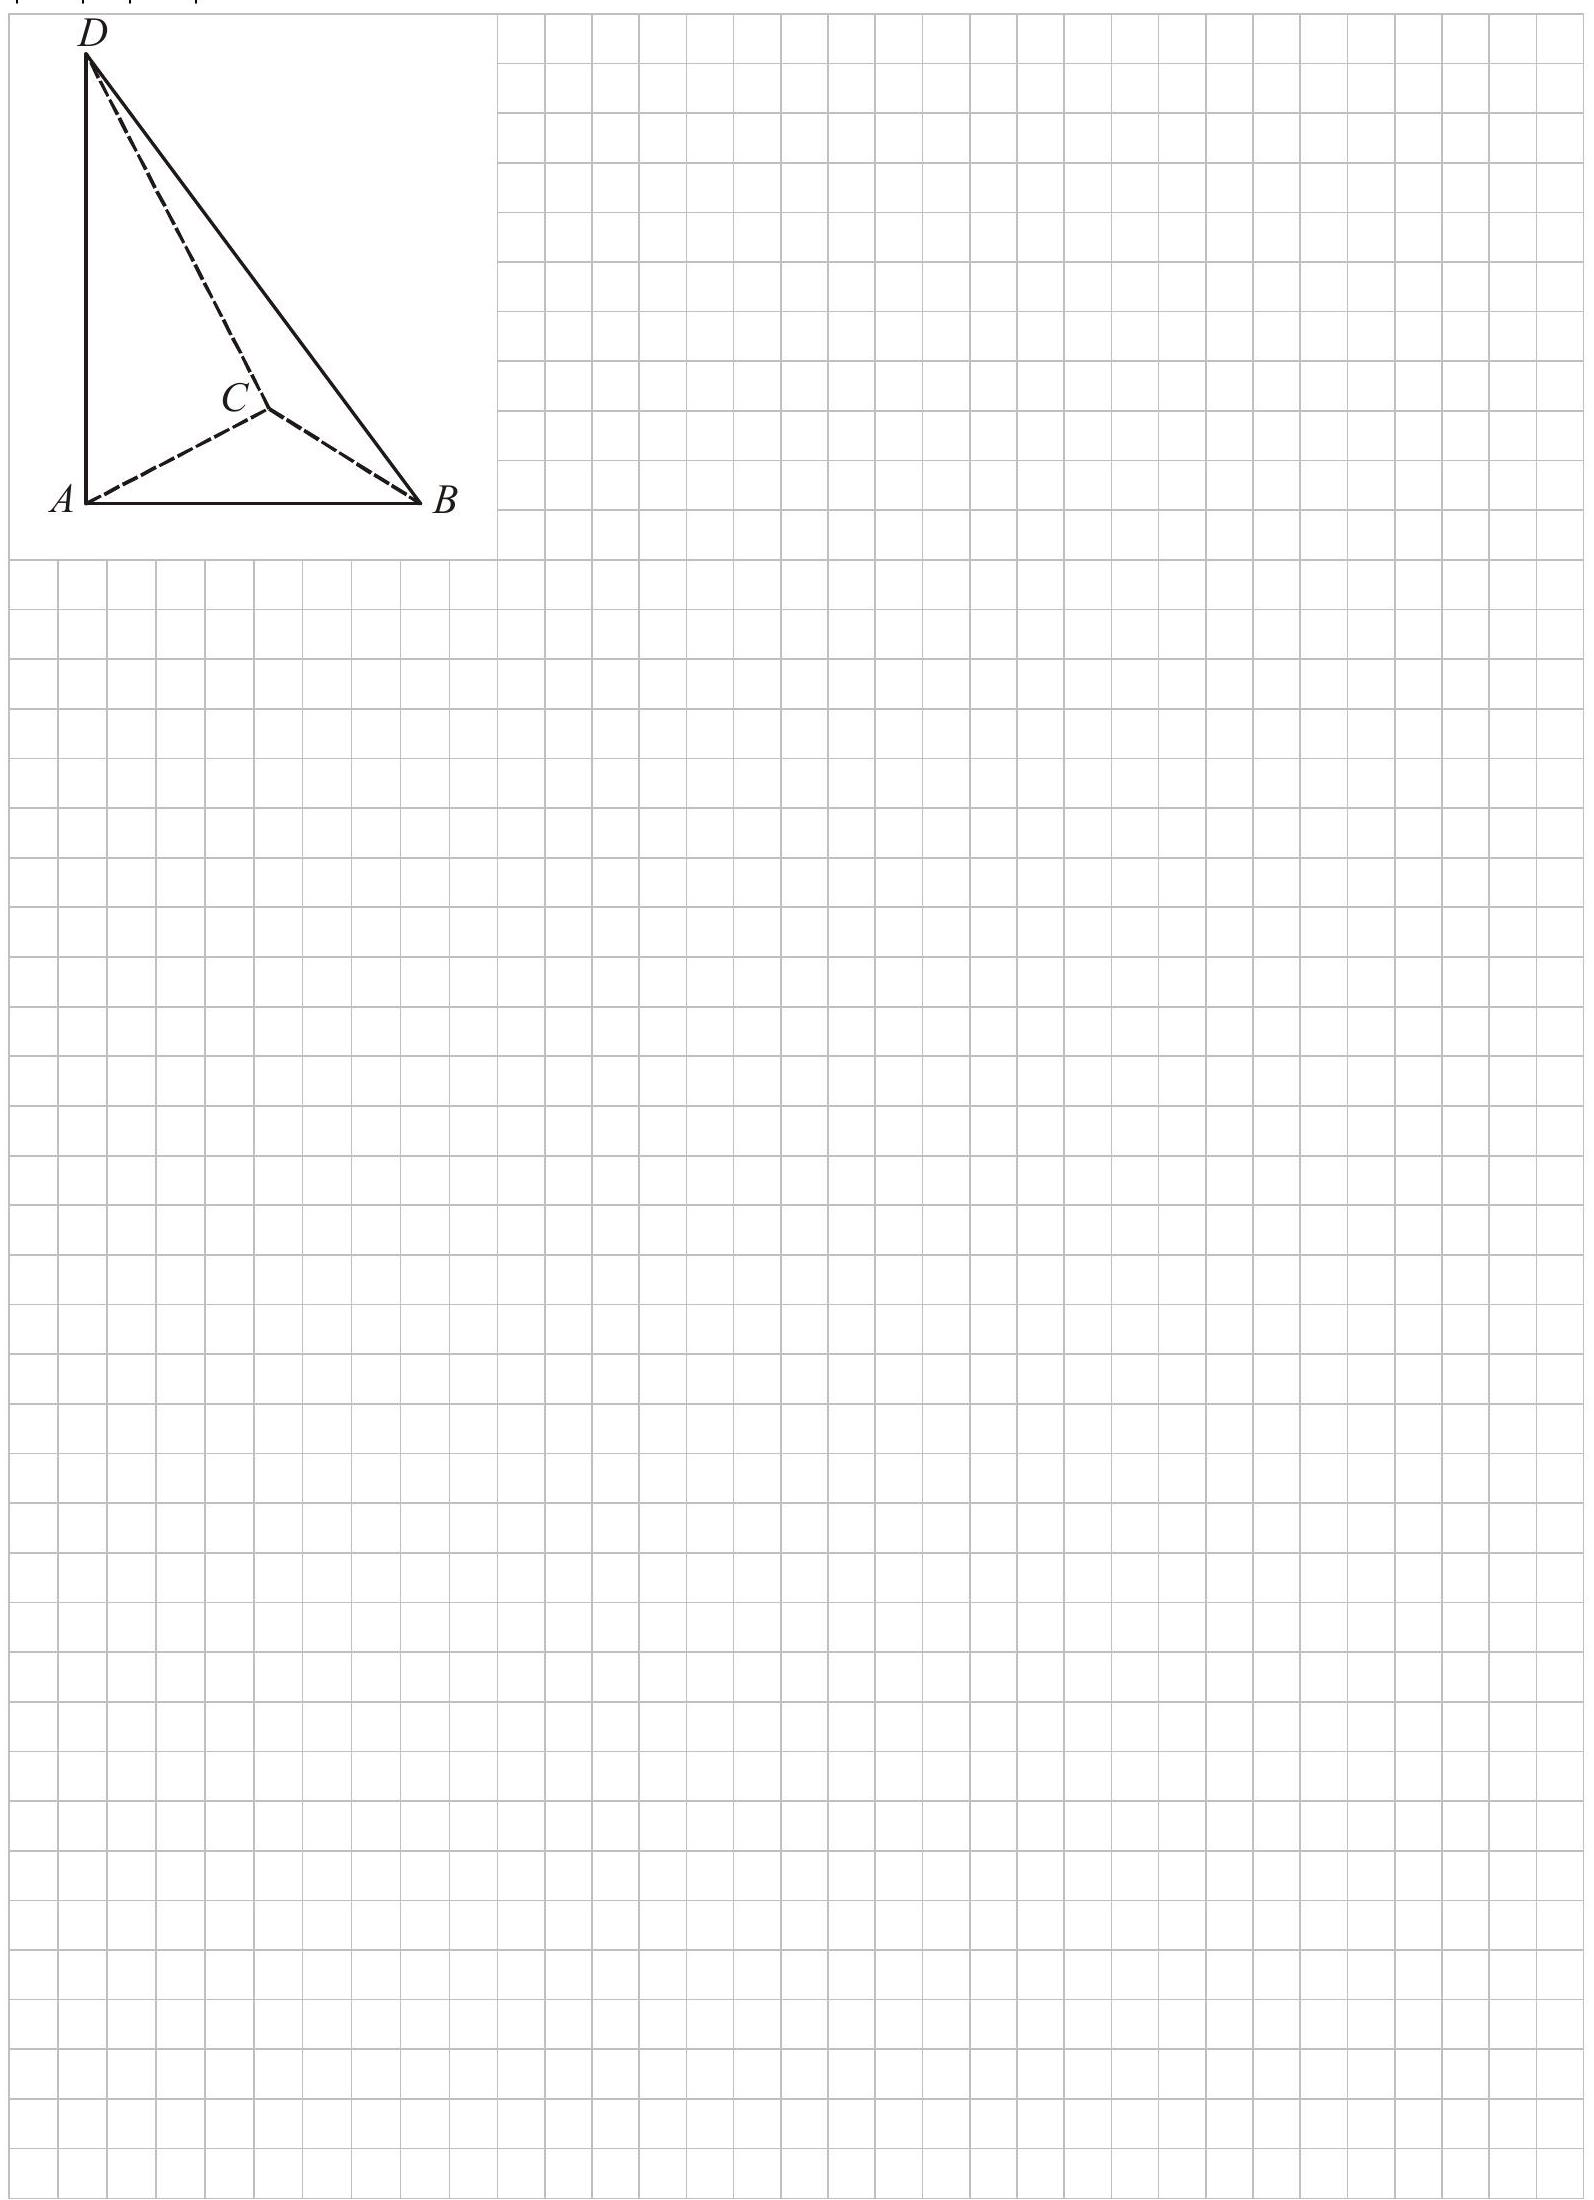
\includegraphics[max width=\textwidth, center]{2024_11_21_caf6b2e64dd65c9b24eeg-14}\\

\includegraphics[max width=\textwidth, center]{2024_11_21_caf6b2e64dd65c9b24eeg-15}

Odpowiedź:

\begin{center}
\begin{tabular}{|c|l|c|}
\hline
\multirow{2}{*}{\begin{tabular}{l}
Wypelnia \\
egzaminator \\
\end{tabular}} & Nr zadania & 32. \\
\cline { 2 - 3 }
 & Maks. liczba pkt & 4 \\
\cline { 2 - 3 }
 & Uzyskana liczba pkt &  \\
\hline
\end{tabular}
\end{center}

\section*{Zadanie 33. (4 pkt)}
Doświadczenie losowe polega na dwukrotnym rzucie symetryczną sześcienną kostką do gry. Oblicz prawdopodobieństwo zdarzenia \(A\) polegajacego na tym, że w pierwszym rzucie otrzymamy parzystą liczbę oczek i iloczyn liczb oczek w obu rzutach będzie podzielny przez 12. Wynik przedstaw w postaci ułamka zwykłego nieskracalnego.\\

\includegraphics[max width=\textwidth, center]{2024_11_21_caf6b2e64dd65c9b24eeg-16}\\

\includegraphics[max width=\textwidth, center]{2024_11_21_caf6b2e64dd65c9b24eeg-17}

Odpowiedź:

\begin{center}
\begin{tabular}{|c|l|c|}
\hline
\multirow{2}{*}{\begin{tabular}{c}
Wypetnia \\
egzaminator \\
\end{tabular}} & Nr zadania & 33. \\
\cline { 2 - 3 }
 & Maks. liczba pkt & 4 \\
\cline { 2 - 3 }
 & Uzyskana liczba pkt &  \\
\hline
\end{tabular}
\end{center}

\section*{Zadanie 34. (5 pkt)}
W dwóch hotelach wybudowano prostokątne baseny. Basen w pierwszym hotelu ma powierzchnię \(240 \mathrm{~m}^{2}\). Basen w drugim hotelu ma powierzchnie \(350 \mathrm{~m}^{2}\) oraz jest o 5 m dłuższy i 2 m szerszy niż w pierwszym hotelu. Oblicz, jakie wymiary mogą mieć baseny w obu hotelach. Podaj wszystkie możliwe odpowiedzi.\\

\includegraphics[max width=\textwidth, center]{2024_11_21_caf6b2e64dd65c9b24eeg-18}\\

\includegraphics[max width=\textwidth, center]{2024_11_21_caf6b2e64dd65c9b24eeg-19}

Odpowiedź:

\begin{center}
\begin{tabular}{|c|l|c|}
\hline
\multirow{2}{*}{\begin{tabular}{l}
Wypełnia \\
egzaminator \\
\end{tabular}} & Nr zadania & 34. \\
\cline { 2 - 3 }
 & Maks. liczba pkt & 5 \\
\cline { 2 - 3 }
 & Uzyskana liczba pkt &  \\
\hline
\end{tabular}
\end{center}

\section*{BRUDNOPIS}

\end{document}